\documentclass[a4paper, 11pt]{article}

\usepackage[utf8]{inputenc}

\usepackage[T1]{fontenc}

\usepackage[french]{babel}

\usepackage{graphicx}

\usepackage[margin = 1in]{geometry}

\usepackage{fancyhdr}

\usepackage{float}

\usepackage{biblatex}

\usepackage{csquotes}

\addbibresource{references.bib}


\title{\Large LBIO1355 – Rapport de TP \\
\huge La co-évolution entre les Eulophidae et les Cassidinae}


\author{Gashi Vandenhove Elfie & Guyot Léopold & Hiernaux Stéphane}

\date{\today}
\begin{document}
\begin{titlepage}
   \begin{center}
       \vspace*{1cm}

        \LARGE
       \textbf{ LBIO1355 – Rapport de TP}

       \vspace{0.5cm}
       \Large
       La co-évolution entre les Eulophidae et les Cassidinae
            
       \vspace{1.5cm}
        \Large
       \textbf{Gashi Vandenhove Elfie\\ Guyot Léopold\\ Hiernaux Stéphane}

       \vfill
       \vspace{0.8cm}
     
       
\includegraphics[width=0.6\textwidth]{UCLouvain_Logo_Pos_CMJN.pdf}
            
      \large LBIO1355 – Rapport de TP\\
       Université catholique de Louvain-la-Neuve\\
       Belgique\\
       \today
            
   \end{center}
\end{titlepage}


\pagestyle{fancy}
\fancyhead{}\fancyfoot{}
\fancyhead[L]{
\includegraphics[width = 0.2\textwidth]{UCLouvain_Logo_Pos_CMJN.pdf}}
\fancyhead[R]{La co-évolution entre les Eulophidae et les Cassidinae}
\section{Introduction}
Nous savons tous que l’évolution est le mécanisme clé de la diversité des espèces. Au sein de l’évolution, la coévolution est un processus particulier lors duquel deux espèces évoluent en parallèle, influençant l’une et l’autre leur fitness. Dans ce rapport, nous allons étudier les arbres phylogénétiques de deux familles/sous-familles liées par une relation hôte-parasite afin de prouver leur coévolution. Celles-ci sont d’une part Eulophidae, une famille d’insectes hyménoptères parasitoïdes et plus grands représentants de la super-famille des Chalcidoidea, et d’autre part Cassidinae, une sous-famille d’insectes coléoptères de la famille des Chysomelidae. Ces Cassidinae sont souvent dépendants d’une plante hôte spécifique (Cuignet et al. 2007). Du fait de cette propension à toujours se localiser sur les mêmes familles de plantes, les membres de cette sous-famille sont des proies facilement trouvables pour les prédateurs et les parasites, faisant des Cassidinae la famille la plus parasitée au sein des Chrysomelidae. Cette pression sélective aurait donc mené à de nombreuses évolutions défensives à tous stades de développement chez cette famille (Olmstead 1994).
Le but de ce rapport est de prouver la coévolution entre nos deux familles en opposant les arbres phylogénétiques que nous obtiendrons en comparant des séquences d’ADN homologues. Selon la loi de Farenholz, la phylogénie des parasitoïdes et en miroir avec celle de leurs hôtes (Cuignet 2005). Nous allons donc vérifier si c’est bien le cas et à quel point ces arbres sont-ils l’image de l’autre une fois mis en vis-à-vis.


\section{Choix du marqueur pour les Eulophidae}

\subsection{Marqueur : 28S D2, ITS2 ou CytB ?} 

\subsection{Justification ?}

\section{Méthode de construction d'arbre Eulophidae (parasitoïdes)}

\textit{Soyez précis ! Méthode, modèle, … vous pouvez vous aider de captures d’écran. Pensez à justifier vos choix.}

\section{Méthode de construction d'arbre Cassidinae (hôtes)}

\emph{Soyez précis ! Méthode, modèle, … vous pouvez vous aider de captures d’écran. Pensez à justifier vos choix.}

\section{Arbre Eulophidae (parasitoïdes)}
\subsection{Format parenthétique} 
$((Signiphoridae_species1:0.015285,Signiphoridae_species2:0.128462):1.46985,(Horismenus_species3:0.221766,(((Horismenus_species5:0.019111,Horismenus_species6:0.05062)72:0.067935,(Horismenus_species1:0.144536,Horismenus_species2:0.156884)96:0.164364)68:0.061764,((Emersonella_tanigaster:0.092657,(((Emersonella_carballoi:0.026058,Emersonella_nr_carballoi:0.014511)99:0.099119,(Emersonella_albicoxa:0.121503,(Emersonella_rotunda_subtype1:0,(Emersonella_rotunda_subtype3:0.025135,Emersonella_rotunda_subtype2:0.0003)53:0.004206)98:0.069929)72:0.015958)49:0.021809,((Emersonella_niveipes_sub1:0.092929,Emersonella_niveipes_sub2:0.054961)96:0.092457,((Emersonella_varicolor:0.218957,((Emersonella_planiceps_subtype1:0.011964,Emersonella_planiceps_subtype2:0)100:0.060833,(Emersonella_species3_subtype1:0.018041,Emersonella_species3_subtype2:0.068031)99:0.101026)69:0.021096)61:0.0243,(Emersonella_rotunda_subtype4:0.146251,Emersonella_rotunda_subtype5:0.097387)16:0.016969)47:0)40:0.00721)67:0.017421)72:1e-06,((((Emersonella_reticulata:0.217408,Emersonella_windsori:0.201281)41:0.0354,(Emersonella_nr_hastata:0.247184,(Emersonella_planiscuta:0.292321,(Emersonella_horismenoides_sub2:0.078355,(Emersonella_horismenoides_sub1:0,Emersonella_species4:0.018414)94:0.047046)94:0.080812)79:0.067887)70:0.030555)60:0.022807,(Emersonella_pubipennis_sub1:0,Emersonella_pubipennis_sub2:0.01323)100:0.16614)59:0.015063,(Emersonella_species2:0.319133,(Emersonella_species1:0.050373,((Emersonella_cuignetae_subtype1:0.006681,Emersonella_cuignetae_subtype2:0.024551)90:0.005161,Aprostocetus_sp:3.67715)62:0.063493)62:0.09989)79:0.066898)59:0.115077)72:0.188936)95:0.086078):0.0773606)73;
$
\subsection{Graphe :}

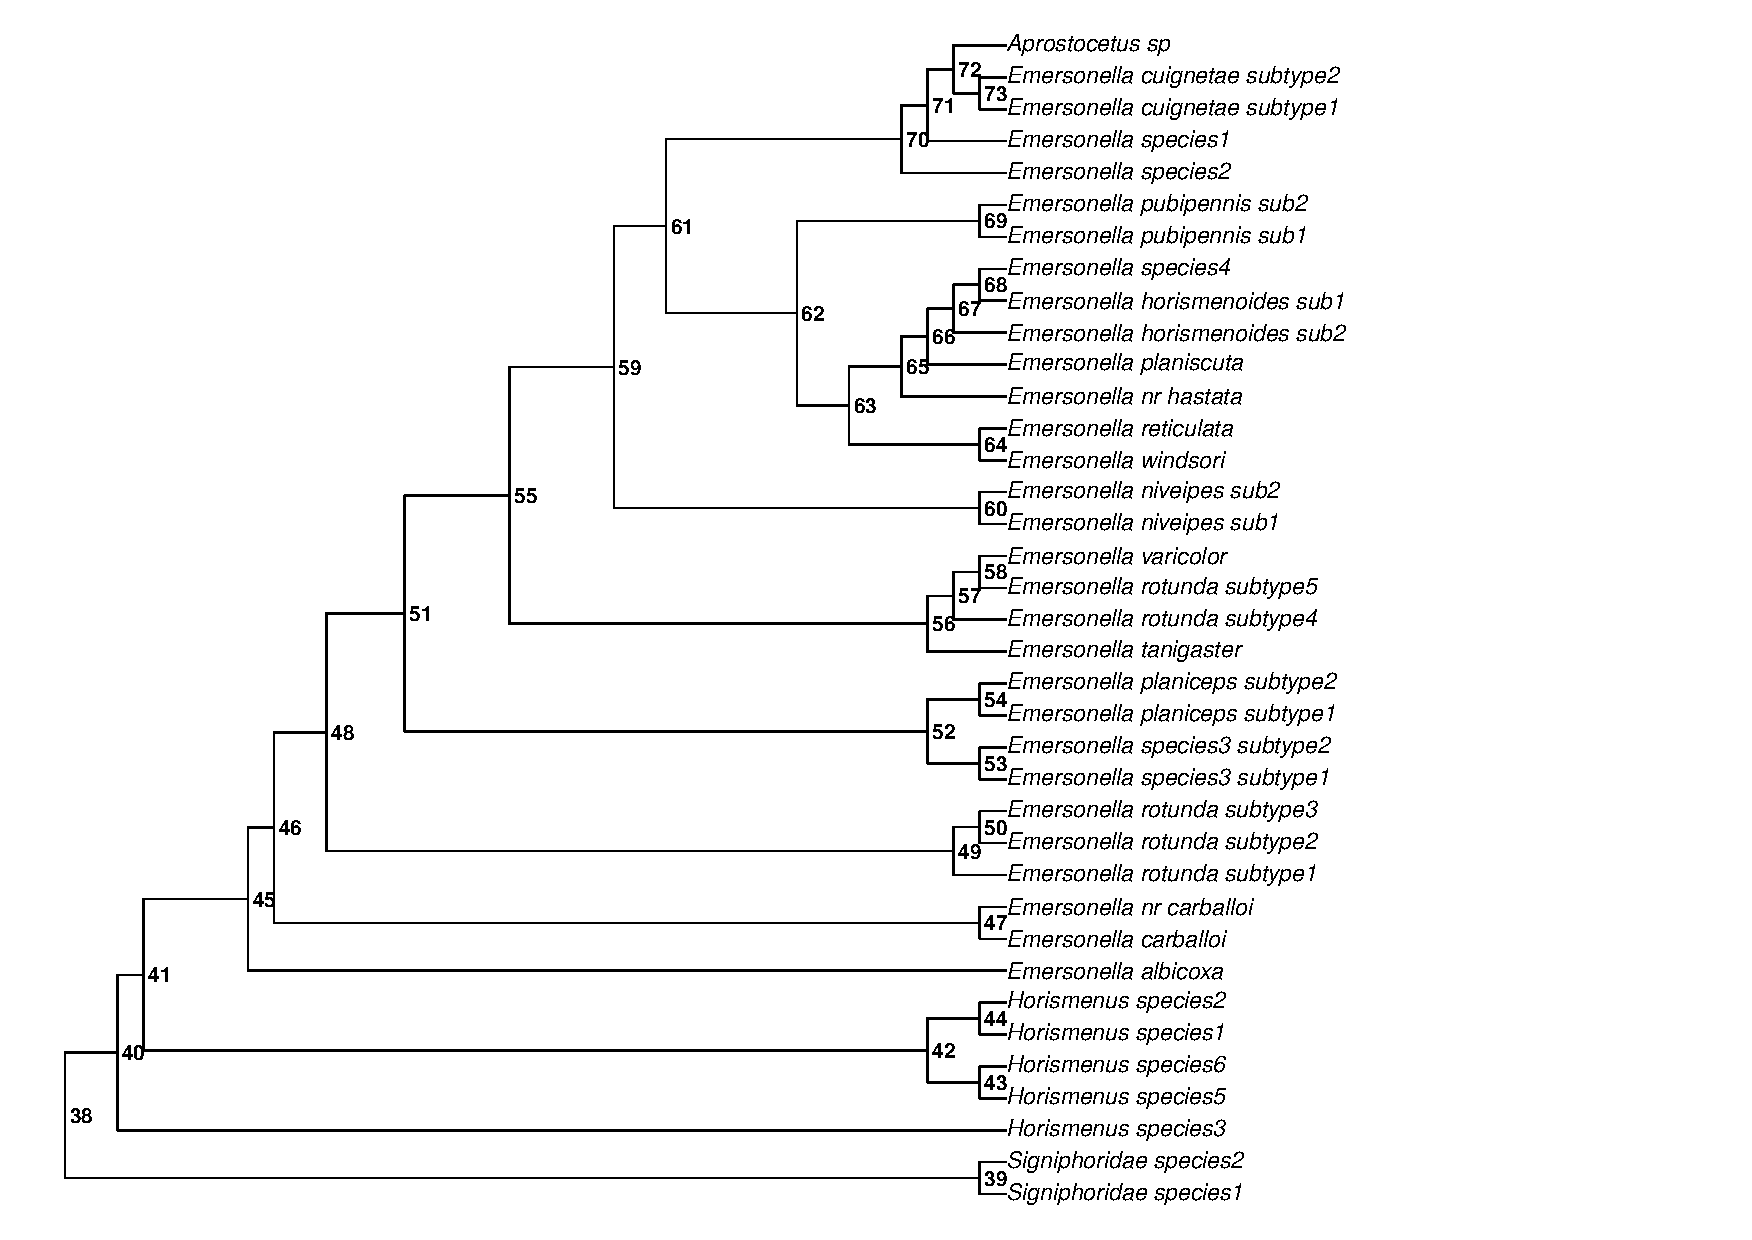
\includegraphics[width = 1\textwidth]{plot_Eulo_Cyt_b_PhyML_GTR_modified.pdf}
\subsection{Discussion}
Tout d’abord, nous pouvons observer que l’outgroup, composé de deux espèces de Signiphoridae, est bel et bien séparé des autres espèces.


Ensuite, on peut observer plusieurs groupements de sous-types d’espèces qui semblent bien agencés, tels que niveipes, species3, planiceps, pubipennis et horismenus. Le groupement rotunda quant à lui est plus dispersé, les subtypes 4 et 5 se trouvant séparés des trois premier qui eux sont tous adjacents. Dans l’arbre réalisé dans l’article de Cuignet de 2005, Aprostocetus semble avoir plus d’ancienneté que là où il est placé dans notre arbre. Nous pouvons donc en déduire que notre arbre n’est pas fiable pour la position de ce genre. On voit également que les subtypes 4 et 5 de rotunda sont bien séparés des trois premiers dans l’arbre de Cuignet, ce qui pourrait indiquer que cette séparation au sein de notre arbre est assez fiable. 


On peut également constater, en comparant notre arbre à celui de Cuignet, que le groupe Horismenus se situe dans les ancêtres communs à la plupart des autres Emersonella, ce qui correspond avec la place que ce groupe tient dans notre arbre. Nos espèces d’Horismenus sont d’ailleurs séparées par deux noeuds, comme chez Cuignet. Cependant l’ordre d’apparition des espèces dans l’arbre ainsi que la manière dont sont agencés ces deux nœuds sont différentes dans notre arbre phylogénétique.


En regardant nos valeurs bootstrap, .... L’arbre de Cuignet semble également avoir une structure différente de la nôtre, mettant en cause la fiabilité de la position de nos genres et espèces. On peut cependant noter plusieurs endroits avec une valeur de bootstrap élevée ainsi qu’une ressemblance avec l’arbre de l’article de Cuignet, telles que l’outgroup Signiphoridae et le groupement assez ancestral et aux espèces adjacentes dans l’arbre de Horismenus. Les valeurs de bootstrap sont également proches de 100 lorsqu’un embranchement débouche sur deux espèces d’un même genre, ce qui est le cas pour les genres niveipes, species3, planiceps, pubipennis et les deux sous-types de cuignetae.
Le fait que les valeurs bootstrap soient aussi peu convaincantes peut être expliqué par le fait que l’analyse se fait sur peu de genres différents, dont le genre Emersonella présent en majorité ayant évolué assez récemment, rendant difficile la différenciation et le placement des espèces dans l’arbre.

\section{Arbre Cassidinae (hôtes)}
\subsection{Format parenthétique} 


\subsection{Graphe :}
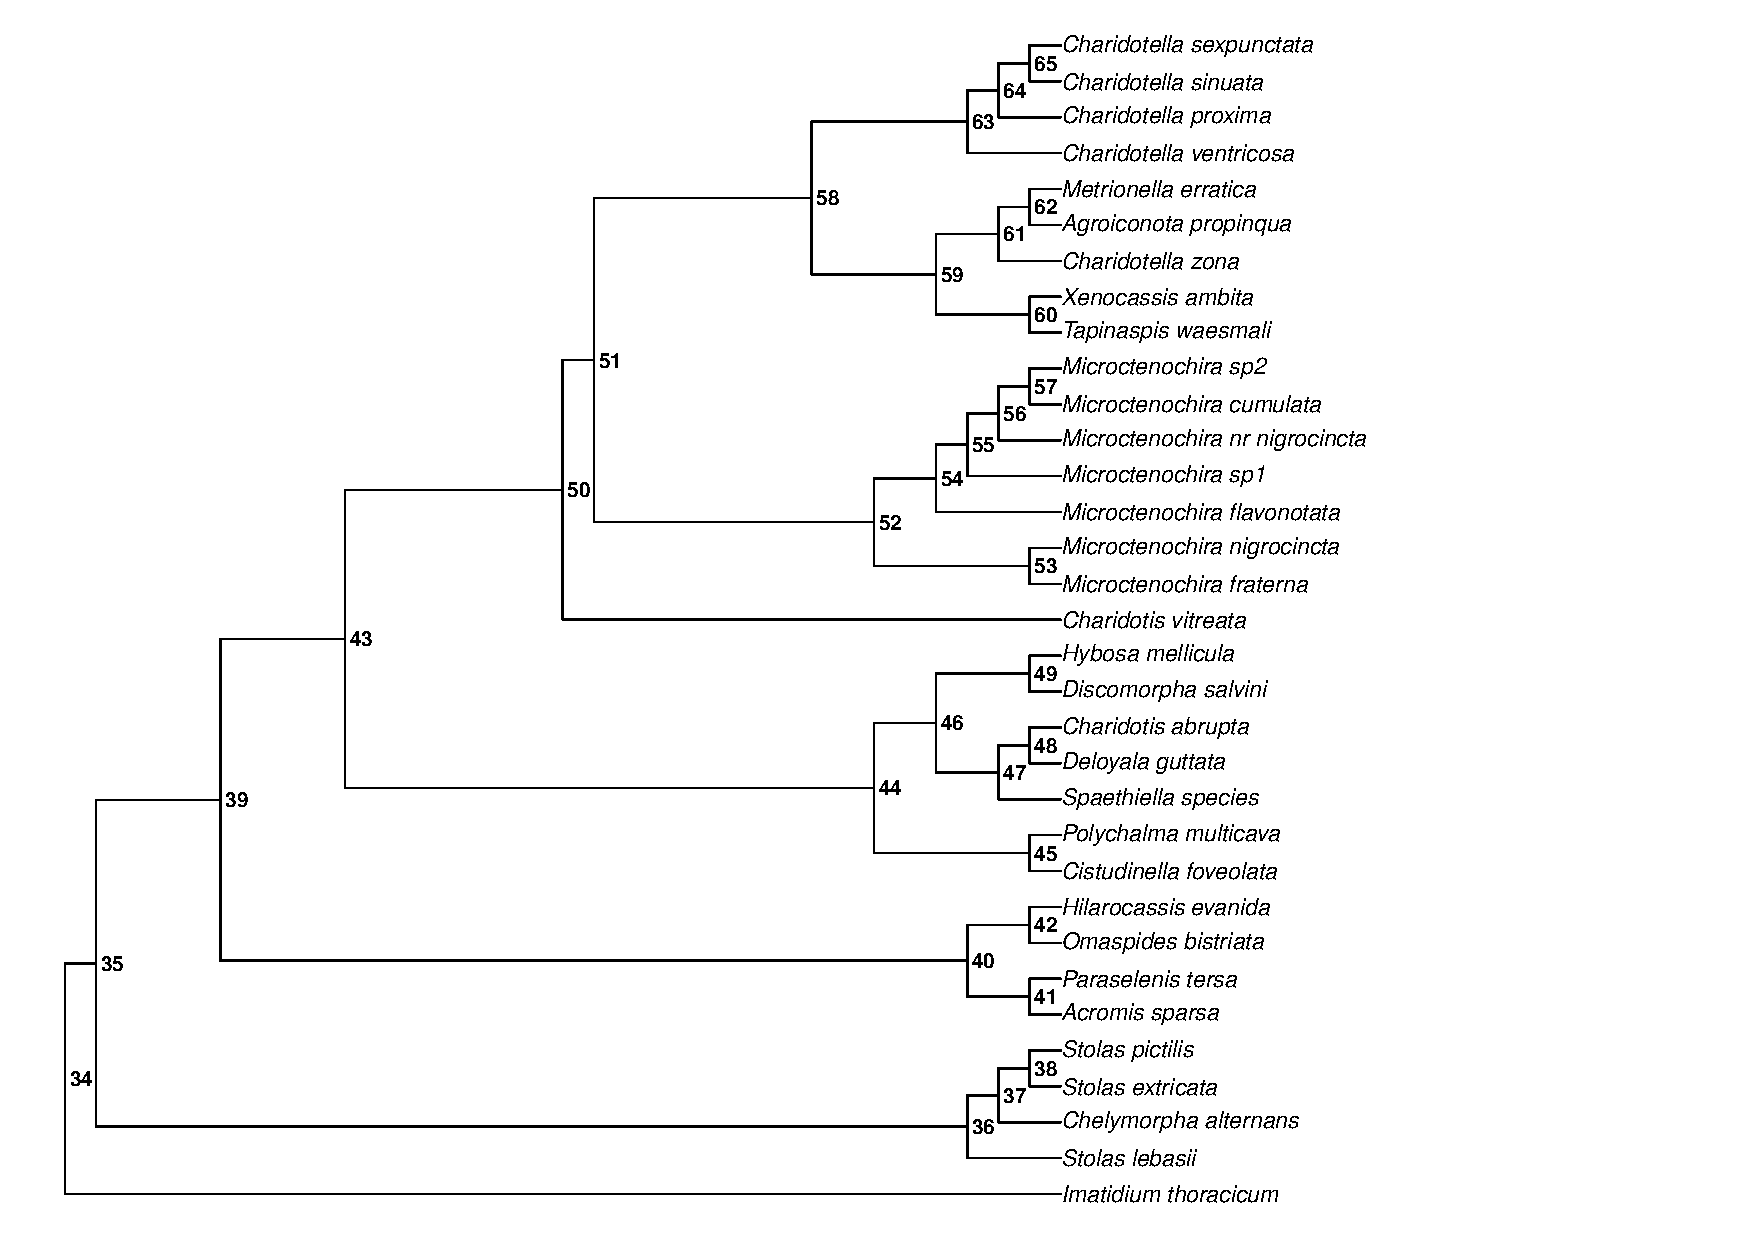
\includegraphics[width = 1\textwidth]{plot_Cassidinae_28S_D2_PhyML_GTR.pdf}
\subsection{Discussion}
\emph{Quelle fiabilité accordez-vous à votre arbre ? De quels regroupements êtes-vous sûrs ou les plus confiants ? Que proposeriez-vous pour améliorer votre résultat ?}
\emph{
Discutez d’abord la topologie sans vous préoccuper des valeurs de bootstraps, puis en en tenant compte.}
\section{Coévolution}

\subsection{Graphe (les deux arbres, et les liens entre eux)}
\emph{Soyez clairs / illustratifs. N’hésitez pas à remettre en forme via R, Powerpoint…}

\subsection{Discussion}
\emph{Y a-t-il selon vous coévolution ? Dans quelle mesure ?}
\section{Conclusion}
\emph{Soyez clairs, concis, synthétiques, cohérents, mais aussi exhaustifs ! La conclusion, c’est la fin de l’histoire, c’est la finalisation du travail. En tant que telle, elle se doit d’en rappeler tous les points importants, de les représenter de manière cohérente, et de montrer ce qu’il a apporté (ce que nous savons en plus et que nous ne savions pas au début). Éventuellement, cette conclusion peut également comprendre une critique constructive et des perspectives.}

\printbibliography

\section{Annexes (.fasta)}

\end{document}
